\documentclass[11pt, aspectratio=43]{beamer}
\DeclareFontShape{OT1}{cmss}{b}{n}{<->ssub * cmss/bx/n}{} 
\usetheme{default}
\usepackage{amsmath}
\usepackage{amsfonts}
\usepackage{mathbbol}
\usepackage{xcolor} % before tikz or tkz-euclide if necessary
\usepackage{tkz-euclide} % no need to load TikZ
\usepackage{multirow}
\usepackage{lmodern}
\usepackage{bm}
\usepackage{caption}
\usepackage{hyperref}
\captionsetup{labelformat=empty,labelsep=none}
\titlegraphic{
\includegraphics[width=2cm]{Figures/UAMS_RGB.png}
}
\usetheme{CambridgeUS}

\title{Biomedical Informatics Research}
\author{Horacio G\'omez-Acevedo, PhD\\ Associate Professor\\Department of Biomedical Informatics\\
	University of Arkansas for Medical Sciences}
\begin{document}
	\begin{frame}[plain]
		\maketitle
	\end{frame}

\begin{frame}{Plan}
	\tableofcontents[hideallsubsections]
\end{frame}

\section{Biomedical Informatics}

\begin{frame}{What is Biomedical Informatics (BMI)}		
	The American Medical Informatics Association (AMIA) gives a broad
	definition of the subject.
	
	{\it
		Biomedical and health informatics applies principles of computer and
		information science to the advancement of life sciences research, health
		professions education, public health, and patient care.}
	\begin{itemize}
		\item BMI develops, studies and applies theories, methods and processes for
		the generation, storage, retrieval, use, and sharing of biomedical data,
		information, and knowledge.
		\item BMI builds on computing, communication and information sciences
		and technologies and their application in biomedicine.
		\item BMI investigates and supports reasoning, modeling, simulation,
		experimentation and translation across the spectrum from molecules to
		populations, dealing with a variety of biological systems, bridging basic
		and clinical research and practice, and the healthcare enterprise
	\end{itemize}
\end{frame}

\begin{frame}{Areas of Research at DBMI}
	As of today, the Department of Biomedical Informatics (DBMI) has four speciality areas
	
	\begin{itemize}
		\item Translational Bioinformatics
		\item Clinical Research Informatics
		\item Imaging Informatics
		\item Clinical Informatics 
	\end{itemize}
	We also have a fellowship in Biomedical Informatics. 
	
	But that is not all! Our faculty has very specific areas of research
	\begin{itemize}
		\item Radiomics, connectomics, neuro-imaging, etc.
		\item Natural Language Processing
		\item Ontologies
		\item Genomics, metagenomics, microbial genomics, cancer genomics, etc.
	\end{itemize}
	
\end{frame}


\begin{frame}{Omics in medicine}
	Since the molecular function is not restricted to the genome, other
	modalities are also informative
	\begin{figure}[h]
		\centering
		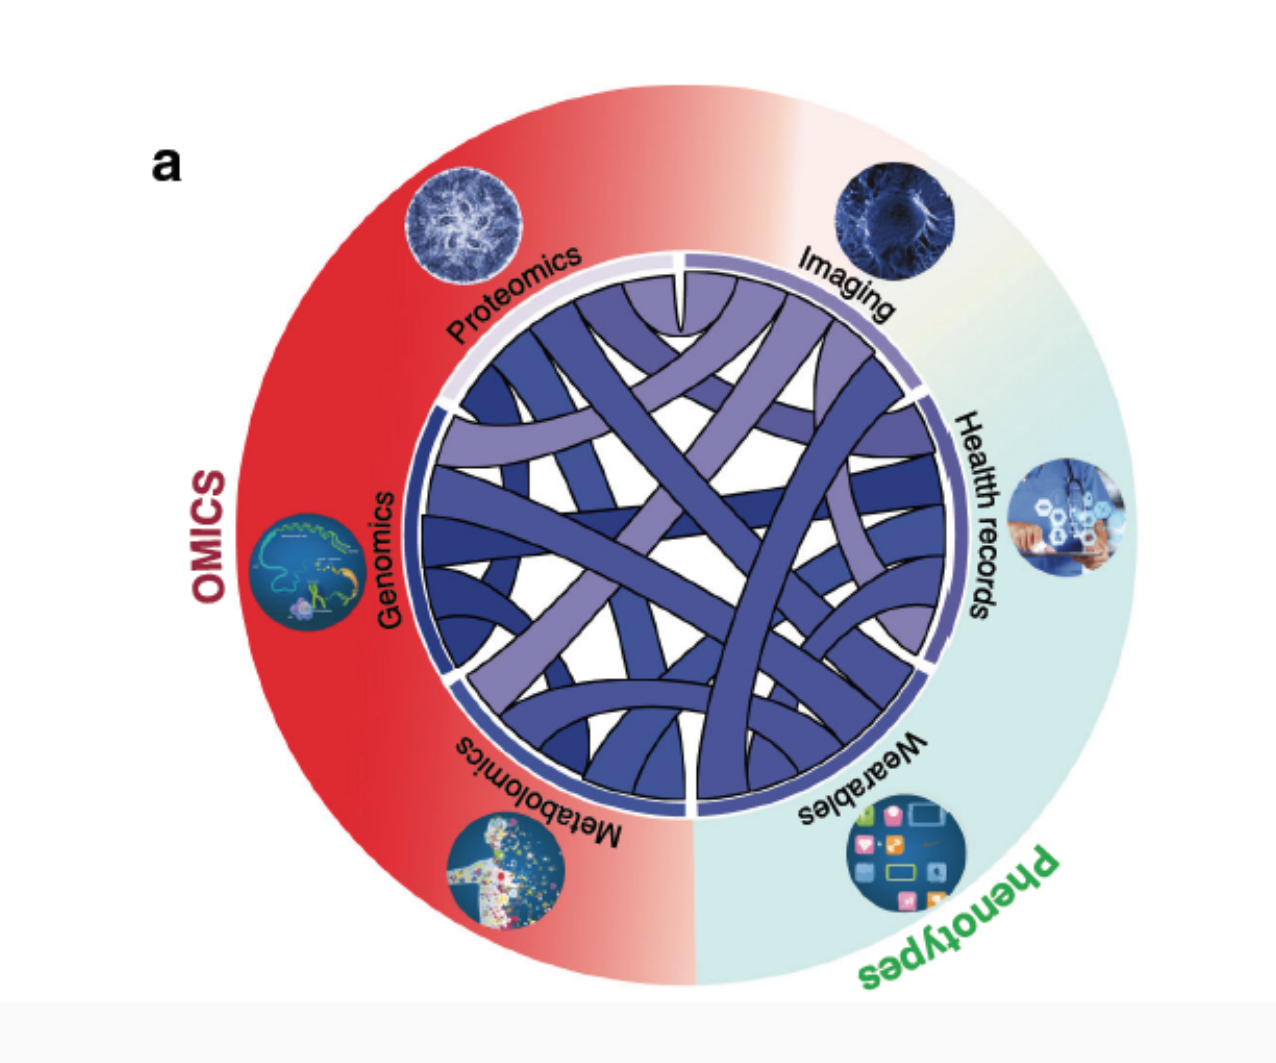
\includegraphics[scale=0.45]{Figures/multiomics.png}
		\caption{Fig 8: Other Omics in healthcare}
	\end{figure}	
	
\end{frame}

\section{Machine Learning}
\begin{frame}{Statistics and traditional parametric approach}
	\begin{figure}[h]
		\centering
		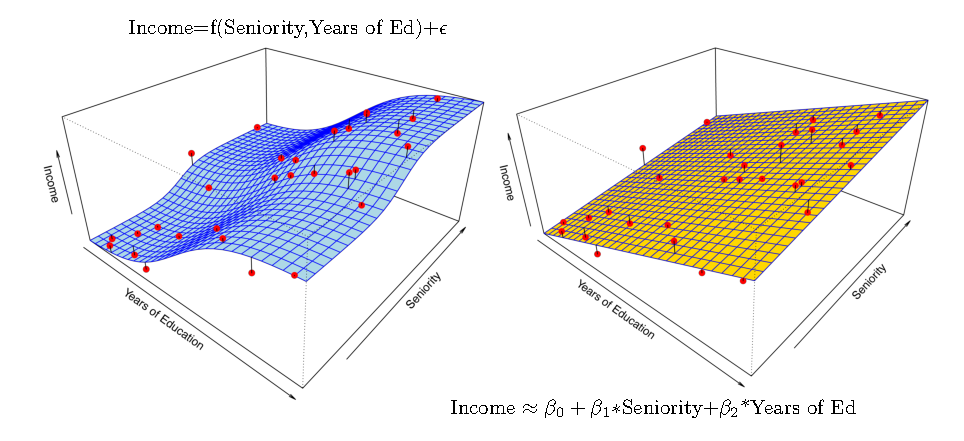
\includegraphics[scale=0.75]{Figures/fig_stat_reg.pdf}
		\caption{Multi-linear regression}
	\end{figure}
\end{frame}




\begin{frame}{Statistics and traditional parametric approach}
	The philosophy of \textit{classical} parametric paradigm is based on three beliefs
	\begin{enumerate}
		\item The functional dependency from the data can be approximated with a linear function with an small number of parameters
		\item Random errors in real life problems follow a normal distribution.
		\item Those parameters  in the model can be calculated via the maximum likelihood method.
	\end{enumerate}
\end{frame}

\begin{frame}{Parametric approach for big data problems}
	\begin{itemize}
		\item 	It was until the computers were introduced that more challenge problems were attempted.
		\item For large multivariate problems, it was observed that increasing the number of factors required more and more computational resources.
		\item R. Bellman called this phenomena the \textbf{curse of dimensionality} 
	\end{itemize}

	New techniques were developed to make informal inferences of data instead of relying in purely statistical techniques. 

\end{frame}

\begin{frame}{Curse of Dimensionality}
	In higher dimensions our intuition is severely impaired
		\begin{figure}[h]
		\centering
		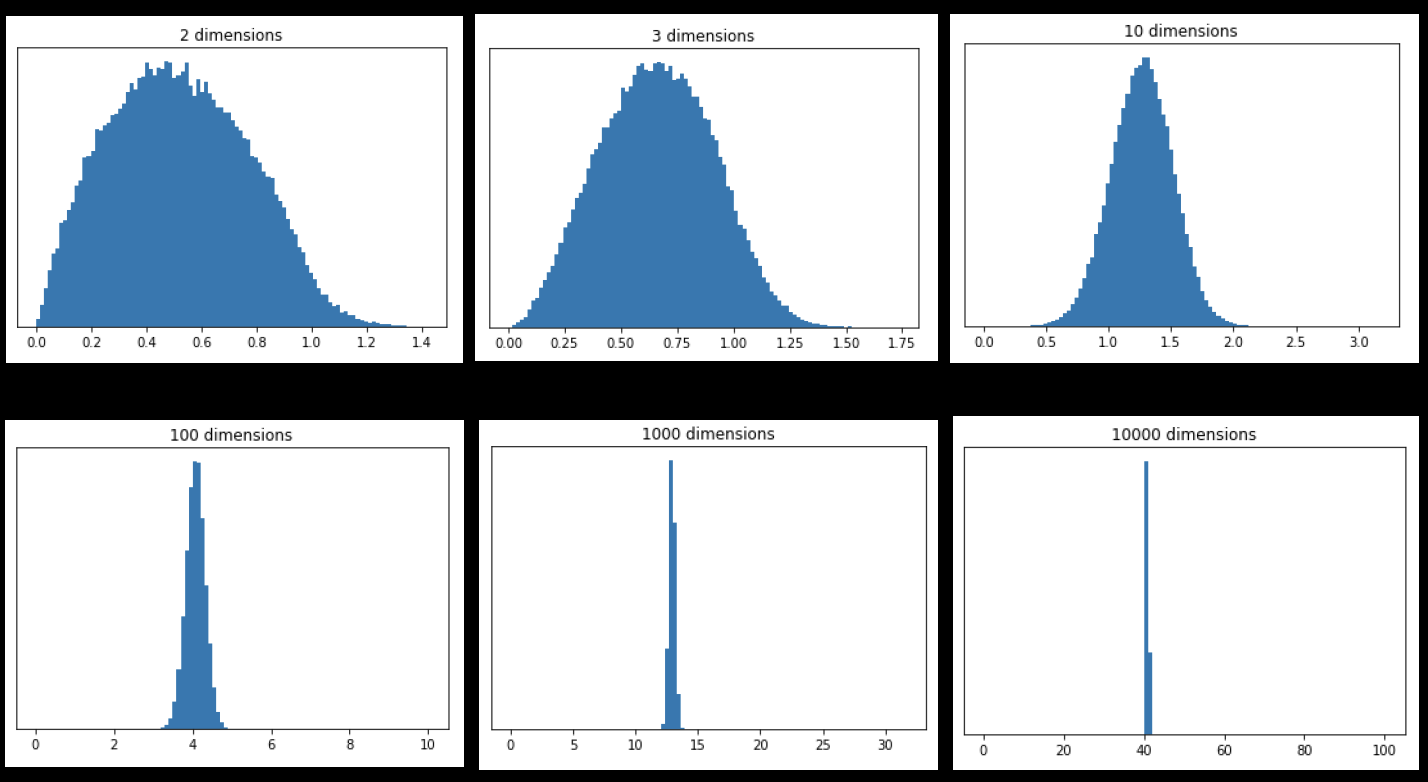
\includegraphics[scale=0.45]{Figures/fig_curse_dim.png}
		\caption{Random vectors in $\mathbb{R}^n$ (Johh Urbanic, Pittsburgh Supercomputing Center)}
	\end{figure}
	
\end{frame}

\begin{frame}{What is Machine Learning?}

	Machine learning (ML) is a vast field and here are some definitions.
	
\begin{quote}
	(ML is the) field of study that gives computers the ability to learn without being explicitly programmed.
	
	Arthur Samuel 1959
\end{quote}	
	
	

\begin{quote}
	A computer program is said to learn from experience E with respect to some task T and some performance measure P, if its performance on T as measured by P, improves with experience E.
	
	Tom Mitchell 1997
\end{quote}



\end{frame}
\begin{frame}{Machine Learning $\ne$ Artificial Intelligence}	
	
	\begin{figure}[h]
	\centering
	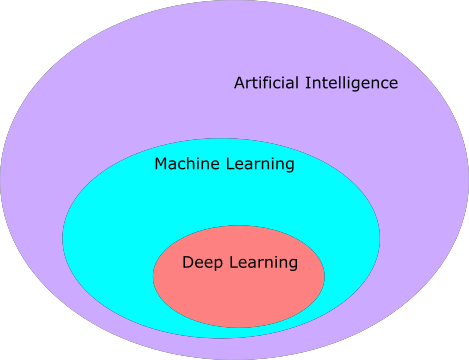
\includegraphics[scale=0.55]{Figures/fig_ml_vs_ai.png}
	%\caption{Multi-linear regression}
\end{figure}
	
\end{frame}

\begin{frame}{When do you use ML?}
	\begin{itemize}
		\item Problems for which existing solutions require a lot of hand-tuning or long lists of rules.
		\item Complex problems for which there is no good solution at all using a traditional approaches.
		\item Fluctuating environments as Machine Learning systems can adapt to not previously seen data.
		\item \textbf{Getting insights about complex problems and large amounts of data.}	
	\end{itemize}

\end{frame}
	

\begin{frame}{Types of ML algorithms}
		
	ML algorithms can be classified according to the amount and type of supervision is required during training. There are fundamentally four major categories: 
	\begin{enumerate}
		\item supervised
		\item unsupervised
		\item semisupervised
		\item reinforced learning
	\end{enumerate}
	
\end{frame}

\begin{frame}{Supervised Learning}
	
	In Supervised Learning, the training data you feed the algorithm includes the desired solutions (called \textbf{labels}).
	
\begin{itemize}
	\item \textbf{Classification}. Algorithm is trained with samples along with their class, and we select parameters that discerns best the labels.
	\item \textbf{Regression}. Algorithm is trained and predict a target numeric value given a set of features (covariates or predictors).
\end{itemize}

Depending on the data set or problem, we divide our sample in three classes:
\begin{itemize}
	\item Training set. A subset in which the algorithm will fit the best model.
	\item Testing set. A subset in which our measures of performance will be used.
	\item Validation set. Ideally, and independent set that will see how our model performs in not-previously seen data.
\end{itemize}
	

\end{frame}


\begin{frame}{Supervised Learning (cont)}
	
	
	Other supervised learning algorithms include
	\begin{itemize}
		\item 	Multilinear (logistic) regression
		\item 	Suport Vector Machines (SVMs)
		\item 	Decision Trees and Random Forest
		\item  Linear Discriminant Analysis
	\end{itemize}


\end{frame}

\begin{frame}{Basic Classification: Separation by planes}
A very common approach for classification of vectors is to find a (hyper)plane that separates the data
	\begin{figure}[h]
		\centering
		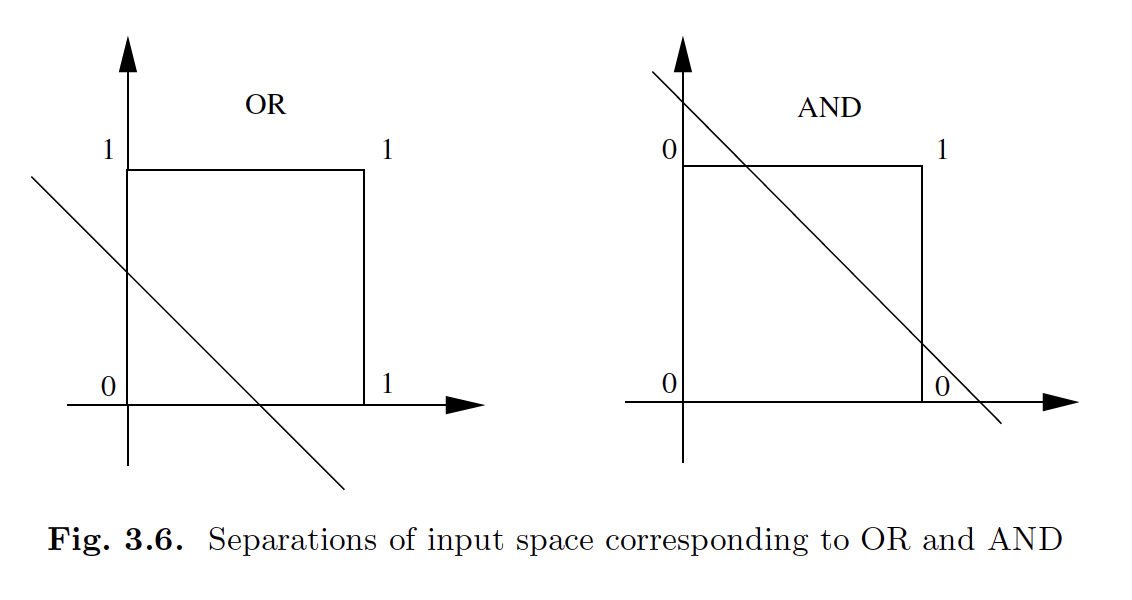
\includegraphics[scale=0.5]{Figures/nn_3.6.png}
		%\caption{Multi-linear regression}
	\end{figure}
	
	
\end{frame}


\begin{frame}{Separation by hyperplanes}
More generally, we separate points (vectors) in higher dimensions with hyperplanes

\begin{figure}[h]
	\centering
	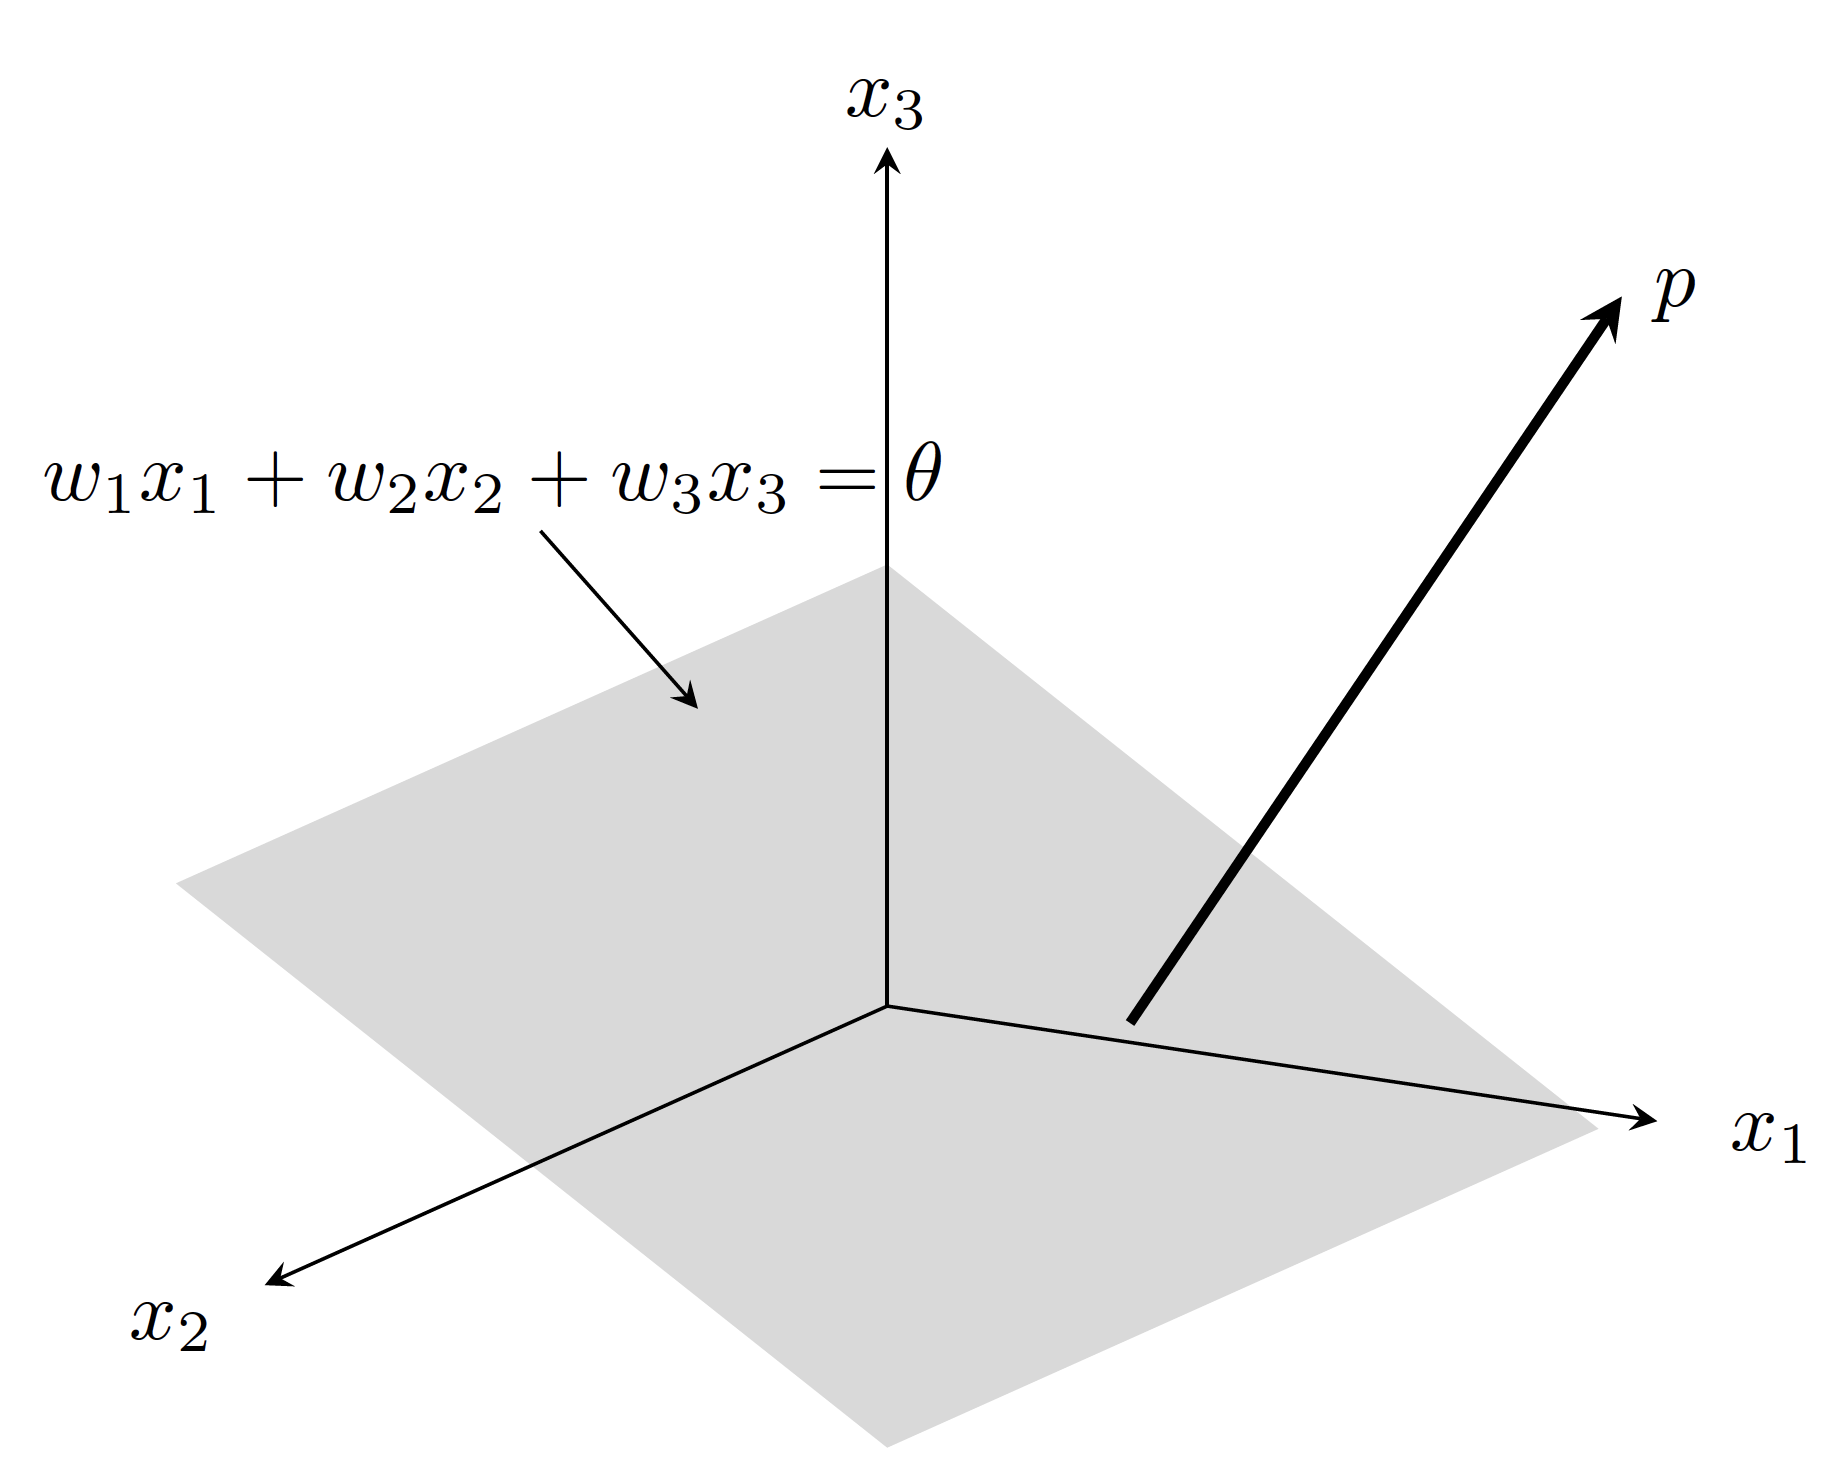
\includegraphics[scale=0.25]{Figures/plane_figure.png}
	%\caption{Multi-linear regression}
\end{figure}

\end{frame}

\begin{frame}{XOR function}
	However, even when we have a relatively simple function XOR this separation is not possible in $\mathbb{R}^2$.
\begin{figure}[h]
	\centering
	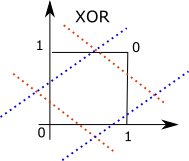
\includegraphics[scale=1.2]{Figures/xor_function.png}
	%\caption{Multi-linear regression}
\end{figure}	
	
\end{frame}

\begin{frame}{Support Vector Machines}
	Using an optimization procedure over the number of misclassified elements close to the hyperplane, we develop another separation algorithm based on the support vectors.
\begin{figure}[h]
	\centering
	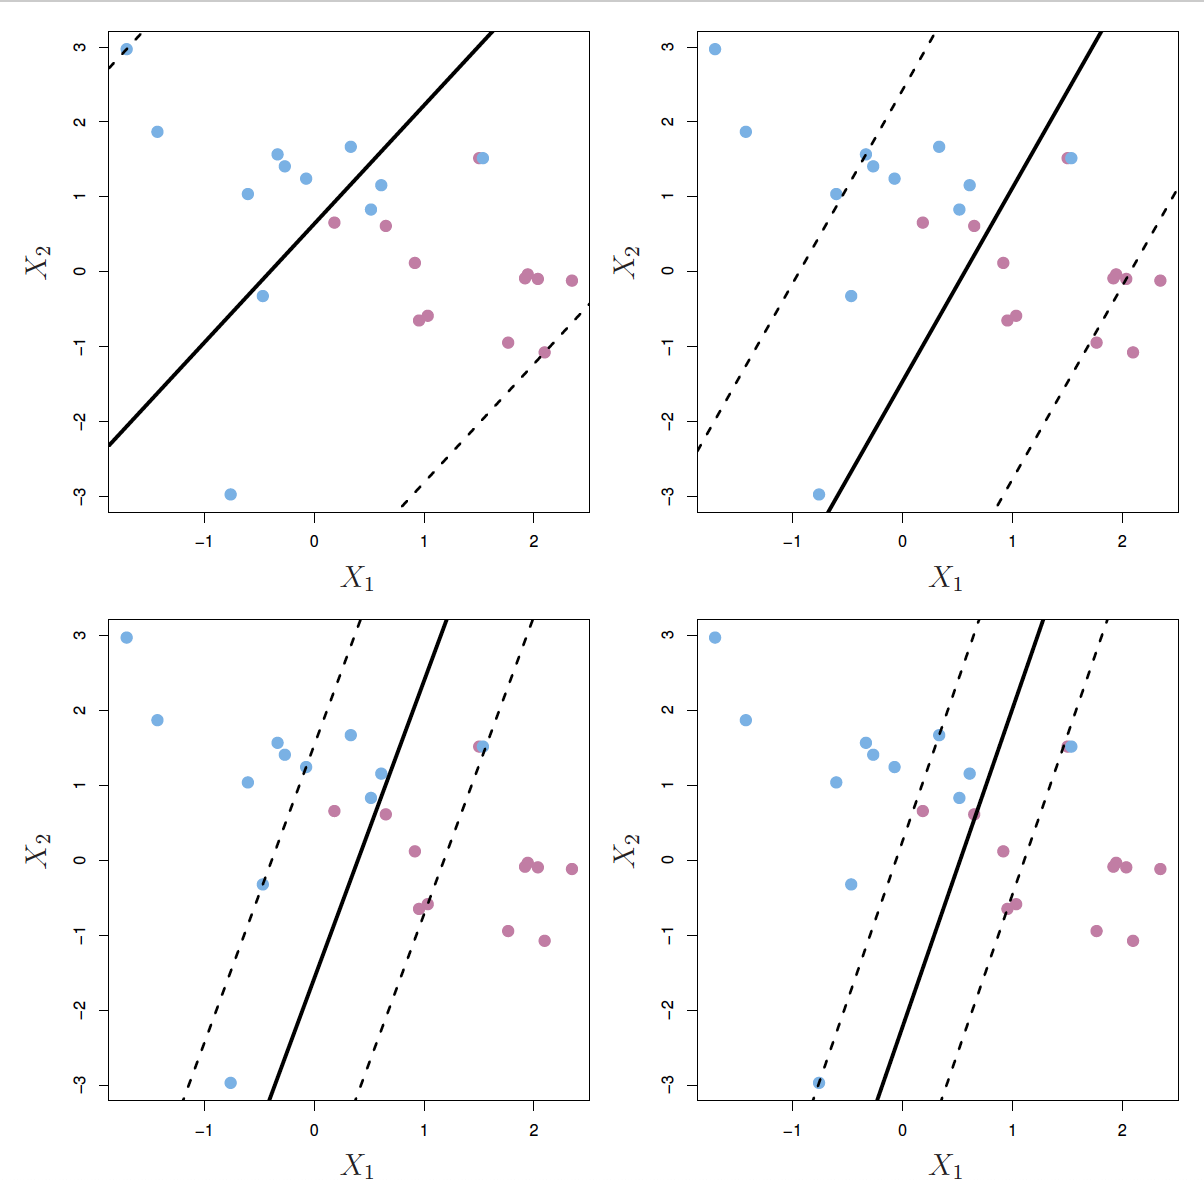
\includegraphics[scale=0.25]{Figures/fig_changing_c_svm.png}
	%\caption{Multi-linear regression}
\end{figure}		
	
\end{frame}

\begin{frame}{Support Vector Machines}
	This methodology allows us to use \textbf{kernels} to better capture the classification.
\begin{figure}[h]
	\centering
	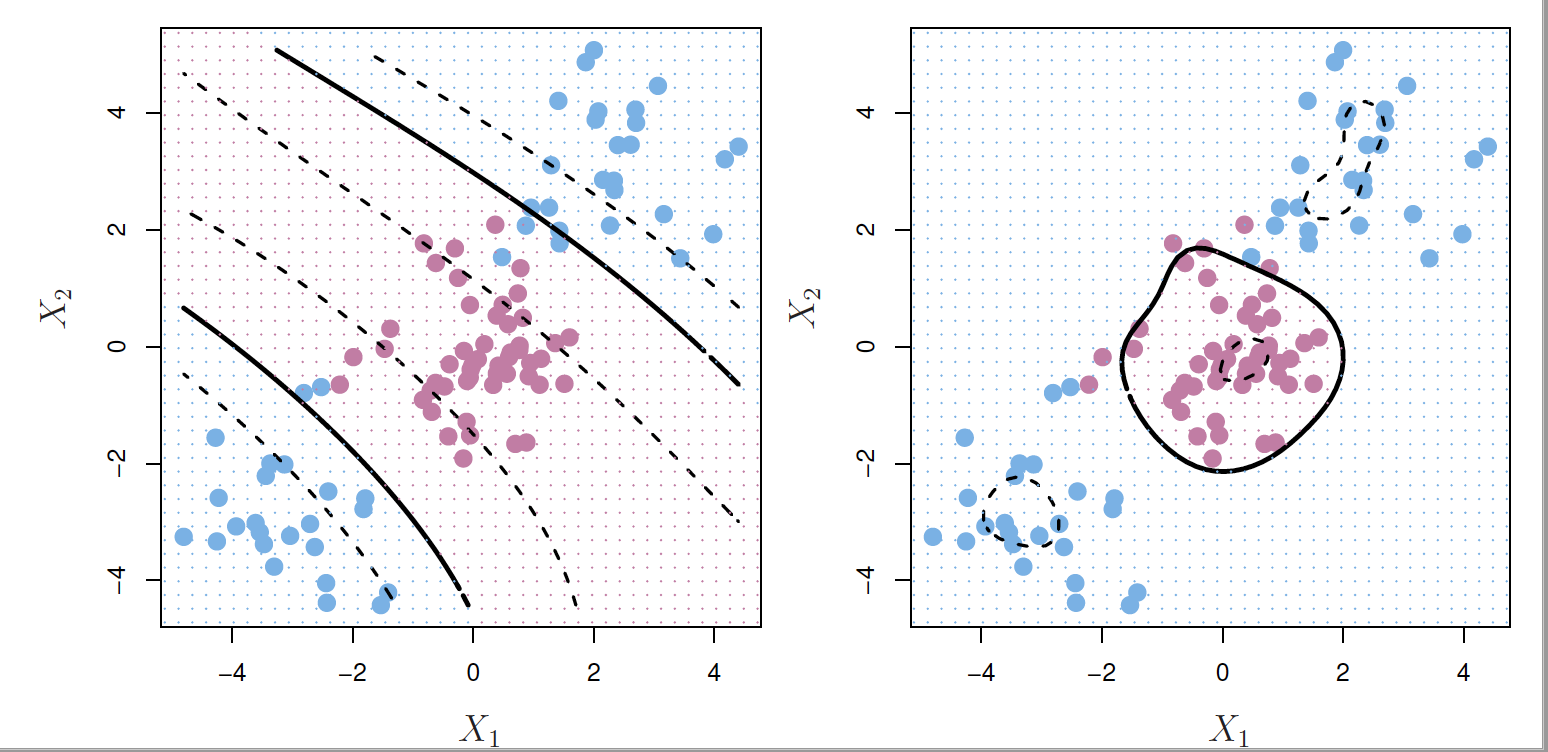
\includegraphics[scale=0.25]{Figures/fig_kernels_svm.png}
	%\caption{Multi-linear regression}
\end{figure}		
	

\end{frame}

\begin{frame}{Tree-based methods}

One of the most intuitive methods for classification is decision trees. 
\begin{figure}[h]
	\centering
	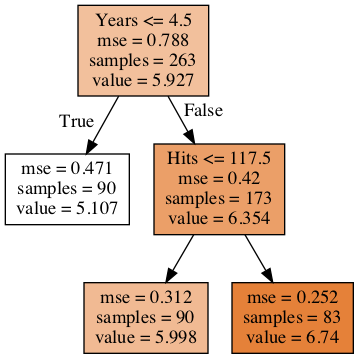
\includegraphics[scale=0.45]{Figures/fig_hitters.png}
	%\caption{Multi-linear regression}
\end{figure}		

\end{frame}

\begin{frame}{Partitions}
	Regression tree based methods have a very simple interpretation .
	
	\begin{figure}[h]
		\centering
		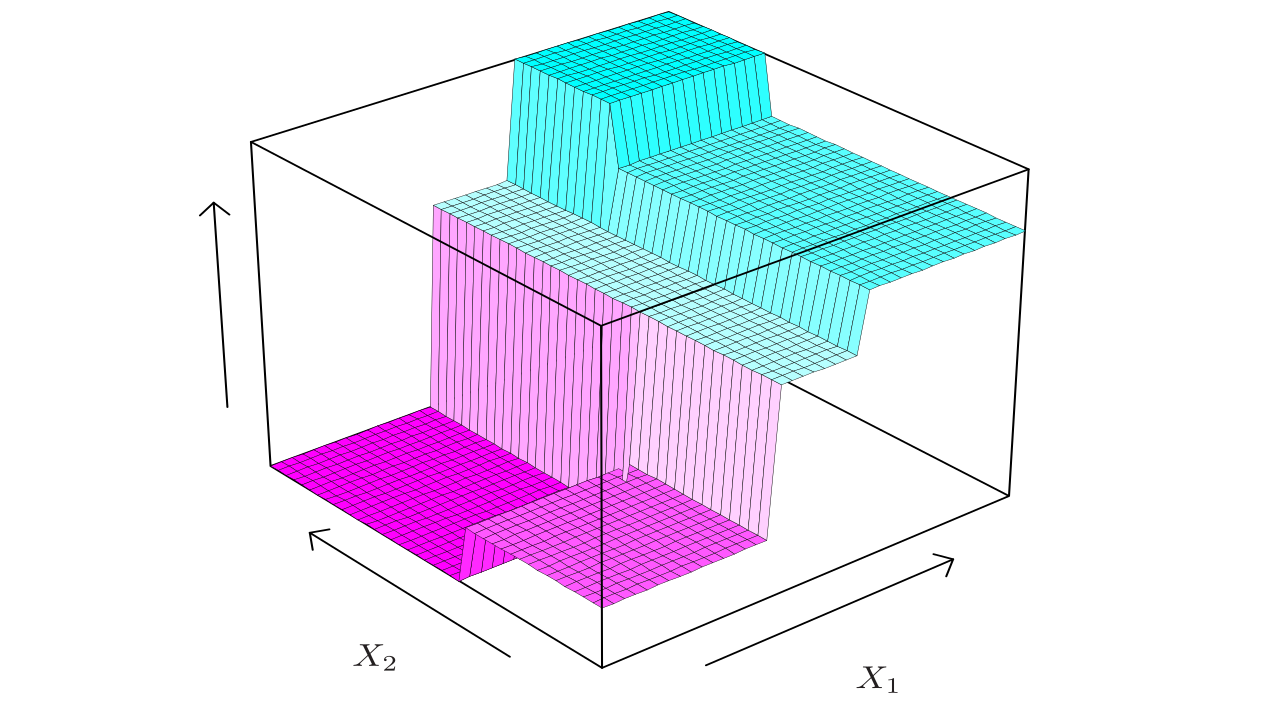
\includegraphics{Figures/3dtreepic.png}
		%\caption{Multi-linear regression}
	\end{figure}		

\end{frame}


\begin{frame}{Random Forest}
	In the setup of classification, we conducted this procedure in two steps
	\begin{enumerate}
		\item Construct binary decision trees using bootstrapped training sets (without pruning)
		\item Predict the value based on the majority vote. That is the class most commonly occurring will be selected. 
	\end{enumerate}	


\end{frame}

\begin{frame}{Trees vs OLS}
	There are some setups where tree methods are more appropriate
	\begin{figure}[h]
	\centering
	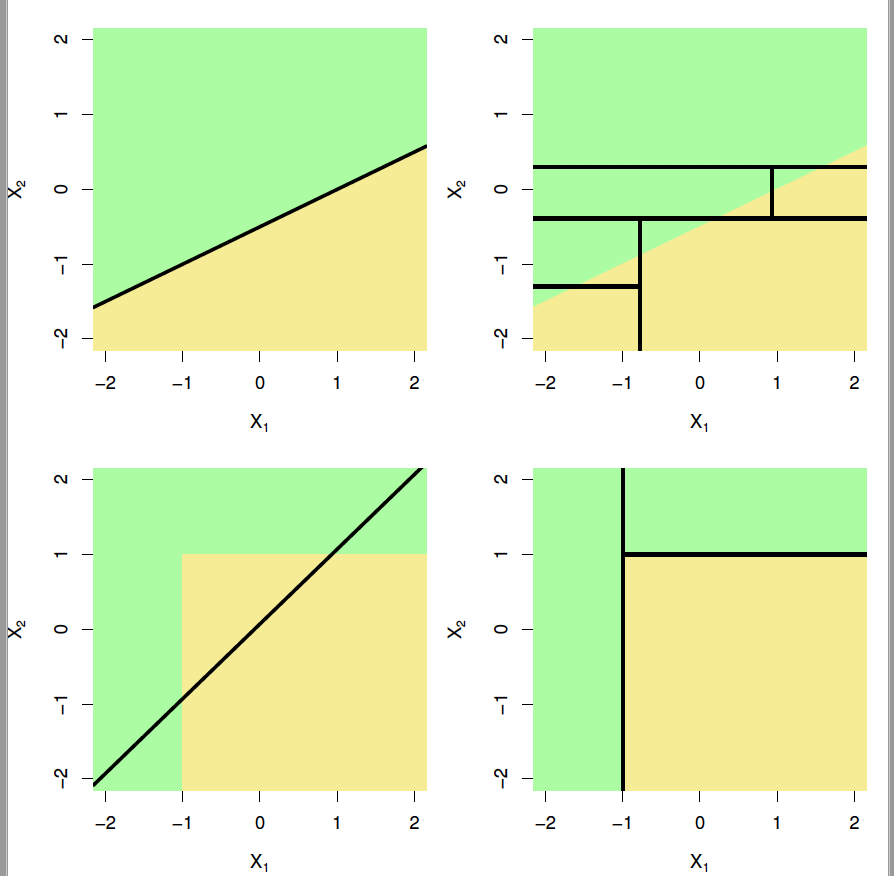
\includegraphics[scale=0.30]{Figures/fig_trees_vs_ols.png}
	%\caption{Multi-linear regression}
\end{figure}			
	
Random forest (boosting/bagging) are very powerful methodologies that compete with regression, their interpretation is complicated.

\end{frame}

%\begin{frame}{Model accuracy}
%Just a quick review of what we called \textit{good fit} in least squares.
%	\begin{figure}[h]
%	\centering
%	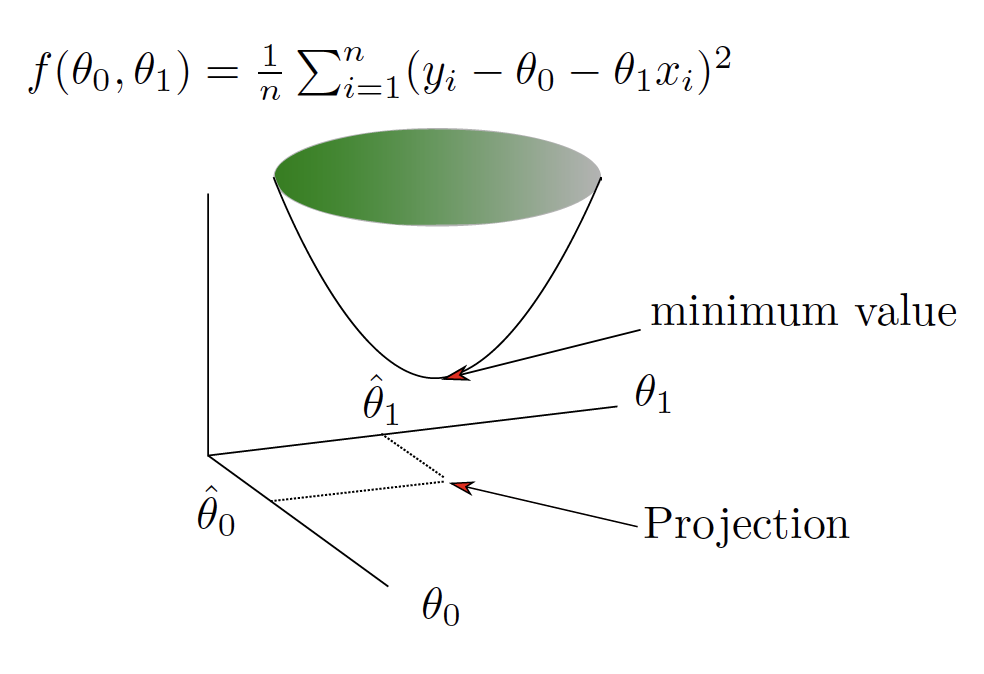
\includegraphics[scale=0.35]{Figures/fig_minfunc.png}
%	%\caption{Multi-linear regression}
%\end{figure}			
%This problem is computationally tracked by using a method called \textbf{gradient descent} to find the minima.
%\end{frame}

\begin{frame}{Unsupervised Learning}	

	In unsupervised learning the training data is unlabeled and the system tries to learn without programmers intervention.
	
	Some of the most important types of unsupervised learning are
	\begin{itemize}
		\item Clustering (K-means)
		\item	Hierarchical Cluster Analysis (HCA)
		\item Visualization and dimensionality reduction
		\begin{enumerate}
			\item 	Principal Component Analysis (PCA)
			\item  Manifold Learning (t-SNE, MDS)
		\end{enumerate}

	\end{itemize}

\end{frame}



\begin{frame}{Clustering}

	The goal of clustering is to detect groups with similar characteristics. If you use hierarchical clustering algorithm it divides each group into smaller subgroups based on certain similarities.
	\begin{figure}[h]
	\centering
	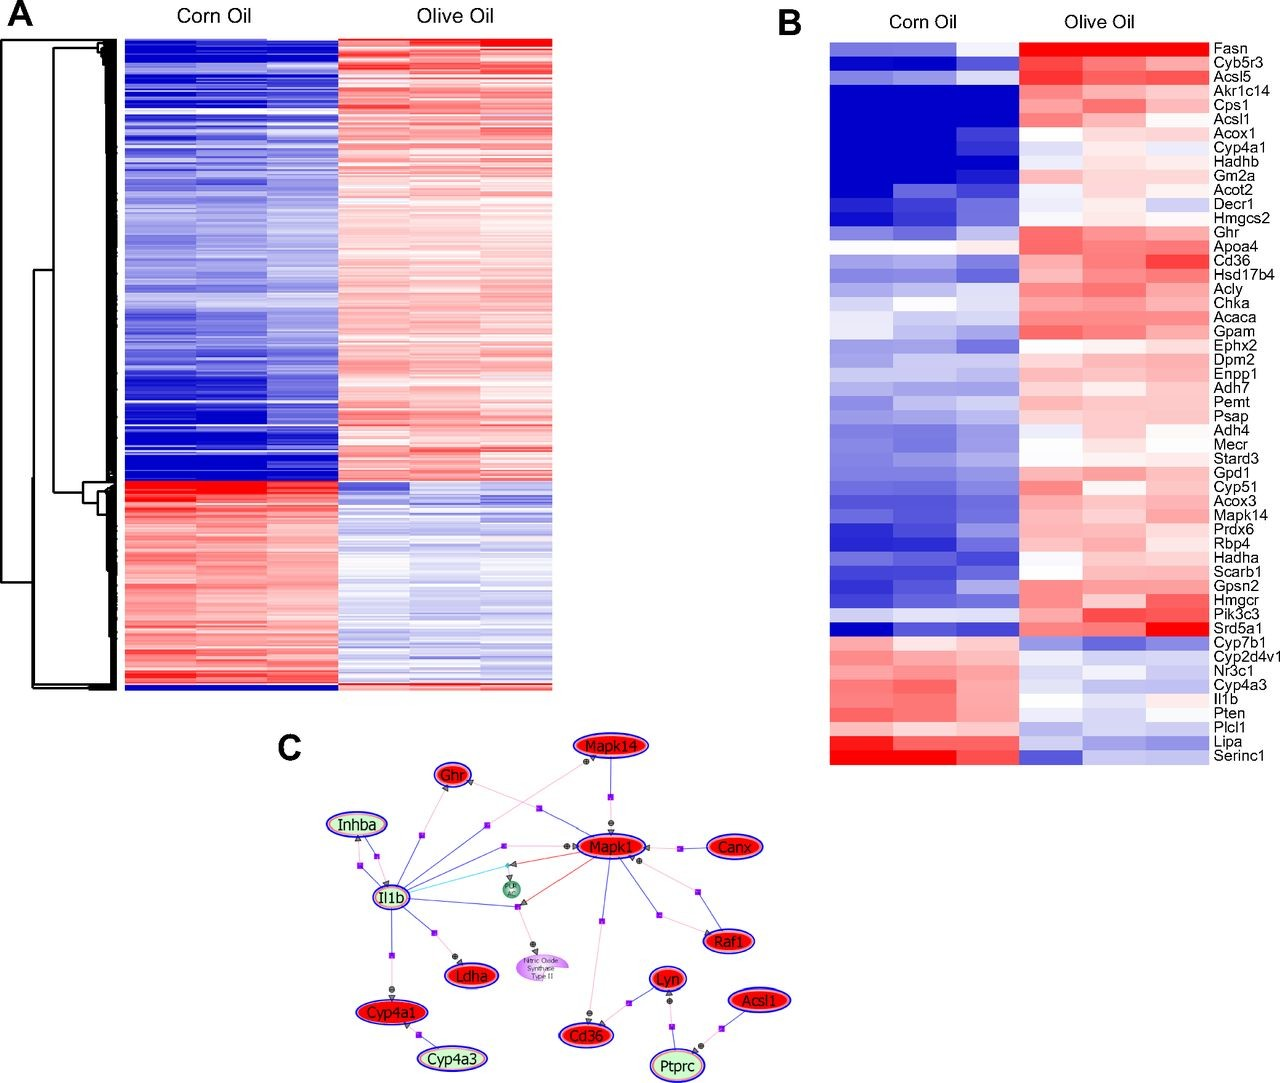
\includegraphics[scale=0.35]{Figures/clustering.jpg}
	%\caption{Multi-linear regression}
\end{figure}			
	

\end{frame}

\begin{frame}{Classification with k-Means Clustering}
	The algorithm goes like this
	
	\begin{enumerate}
		\item Assign randomly a value between 1 and K to each data point.
		\item Iterate the following procedure until the clusters assignments stop changing 
		\begin{enumerate}
			\item  Find the centroid for each of the $K$ clusters.
			\item Each point will be assigned to the cluster $K$ whose distance is the smallest. If two or more are equidistant, select randomly the cluster among the equidistant clusters.
		\end{enumerate}
	\end{enumerate}
	
\end{frame}

\begin{frame}{K-Means Clustering (cont.)}
 
 	\begin{figure}[h]
 	\centering
 	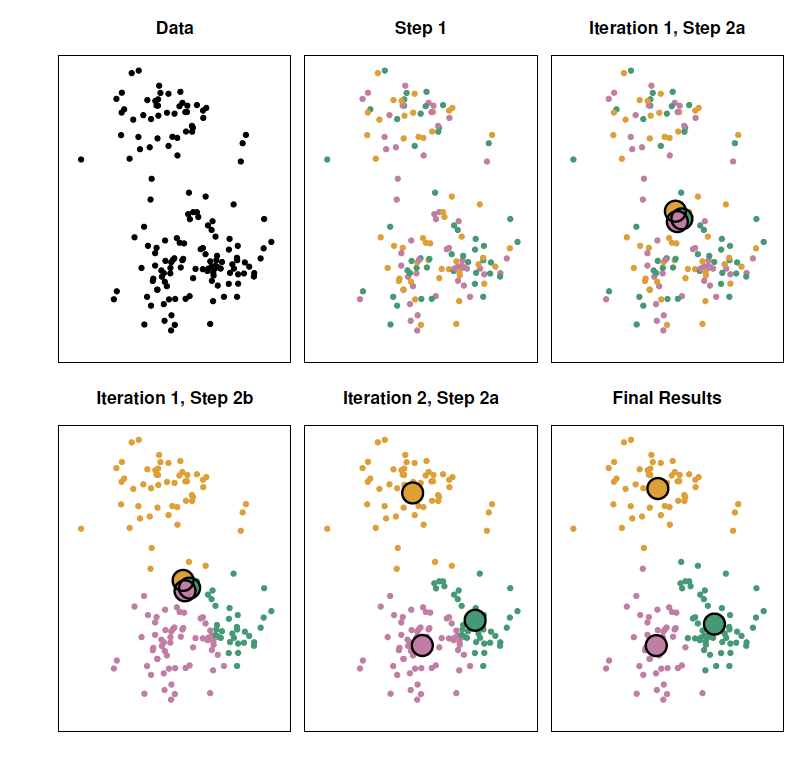
\includegraphics[scale=0.55]{Figures/kmeans_clustering.png}
 	%\caption{Multi-linear regression}
 	\end{figure}
 
\end{frame}

\begin{frame}{PCA}
	The idea of principal component analysis is to reduce the number of dimensions while preserving the data variability. 
	\begin{figure}[h]
		\centering
		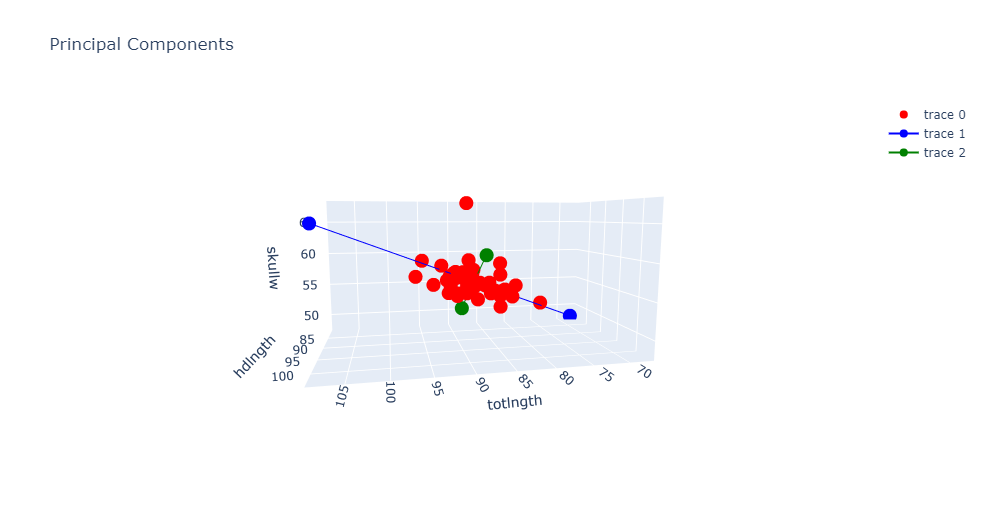
\includegraphics[scale=0.35]{Figures/3d_2pc.png}
		%\caption{Multi-linear regression}
	\end{figure}			
	
\end{frame}


\begin{frame}{Manifold Hypothesis}
		\begin{figure}[h]
		\centering
		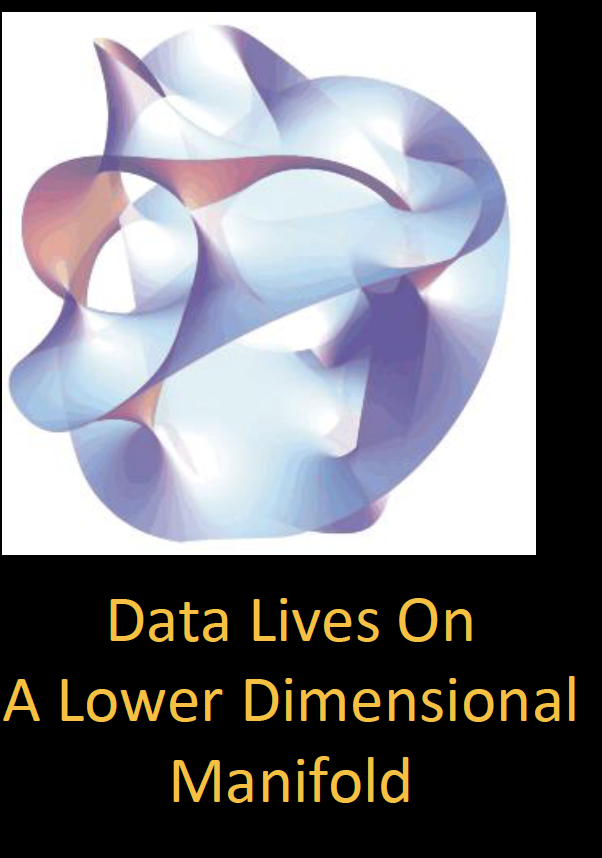
\includegraphics[scale=0.4]{Figures/manifold_hyp.png}
		\caption{John Urbanic, Pittsburgh Supercomputing Center}
	\end{figure}
\end{frame}

\begin{frame}{t-Stochastic Neighbor Embedding}
	This is another methodology that uses the data and their corresponding embedding (projection) and minimizes the Kullback-Leibler divergence of the normalized distribution of the data and their corresponding embedding. 
		\begin{figure}[h]
	\centering
	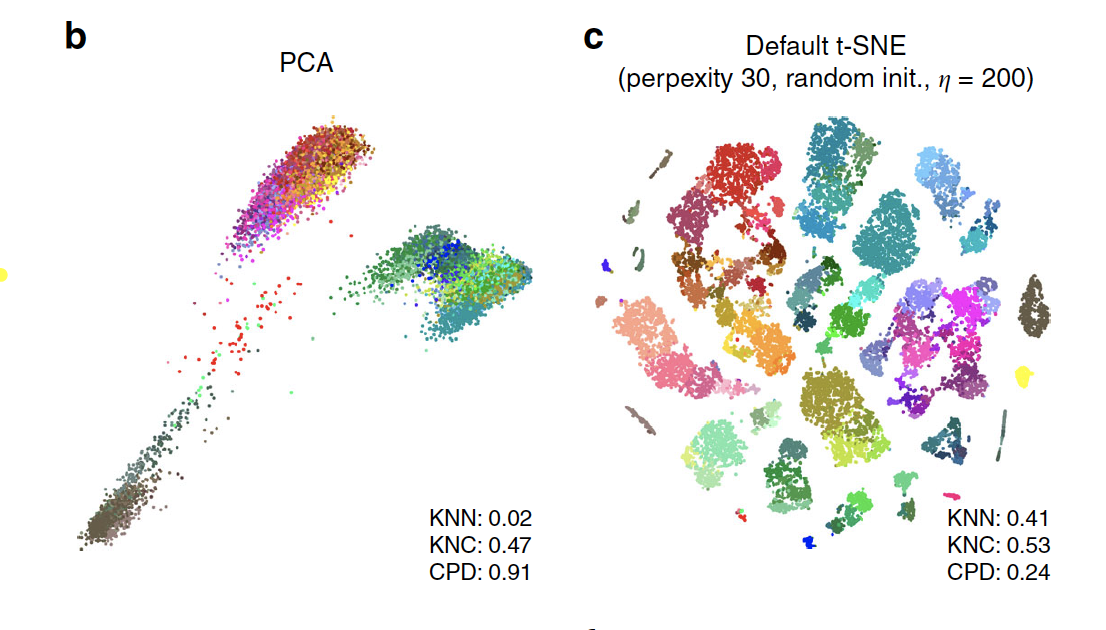
\includegraphics[scale=0.4]{Figures/pca_vs_tsne.png}
%	\caption{John Urbanic, Pittsburgh Supercomputing Center}
\end{figure}	
	
\end{frame}



\begin{frame}{Semisupervised Learning}	

	Algorithms that handle a mixture of labeled and unlabeled data are called semisupervised. As the name suggests, it uses a combination of supervised and unsupervised algorithms. For instance deep belief networks (DBNs) are based on unsupervised components called restricted Boltzmann machines that are trained sequentially in an unsupervised manner, and then the whole system is fine-tuned using supervised learning techniques.

\end{frame}

\begin{frame}{Reinforced Learning}	
	
	The learning system is called an agent in this context, and can observe the environment, select and perform actions and get rewards or penalties. It must then learn by itself what is the best strategy, called a policy, to the most reward over time. A policy defines what action the agent should choose when it is in a given situation. DeepMind's Alpha Go program used reinforced learning to beat world champion Ke Jie at the game of Go. It learned its winning policy by analyzing millions of games, and then playing many games against itself.
\end{frame}

\begin{frame}{Challenges in ML}

	There are either bad algorithms or bad data that can derail any serious ML effort.
	\begin{itemize}
		\item Insuficient quality of training data.
		For very simple problems you typically need thousands of samples, and for complicated such as image or speech recognition you may need millions of samples.
		
		\item Nonrepresentative training data
		To generalize a ML algorithm you need that your training data be representative of the new cases you want to generalize. If the sample is too small, you will have sampling noise, but even very large samples can be nonrepresentative if the sampling method is flawed. This is called sampling bias
	\end{itemize}
	
\end{frame}

\begin{frame}{Challenges in ML (cont)}
	
	\begin{itemize}
		\item 	Poor quality data.
		If your training data is full of errors, outliers and noise, it will make the ML methodology to under perform. Data quality is a field on its own right. Missing features can happen at random or being systematic. Spend enough time with your data to decide quality or features that are missing loads of information.
		\item Overfitting.
		This occurs when the model is too complex relative to the amount and noisiness of the training data. Regularization if the process of reducing overfitting by making the model simpler by introducing a hyperparameter (this is a parameter not for the model but for the algorithm).
	\end{itemize}
	
\end{frame}

\section{Deep Learning}

\begin{frame}{In the beginning... }
	
	In 1958 Frank Rosenblatt proposed the \textbf{perceptron} which is a more general computational model. The essential innovation was the introduction of numeral weights and a special interconnection pattern. In the original Rosenblatt model the computing units are threshold elements and the connectivity is determined stochastically. Learning takes place by adapting the weights of the network with a numerical algorithm. The so-called classical perceptron is depicted below
	
			\begin{figure}[h]
		\centering
		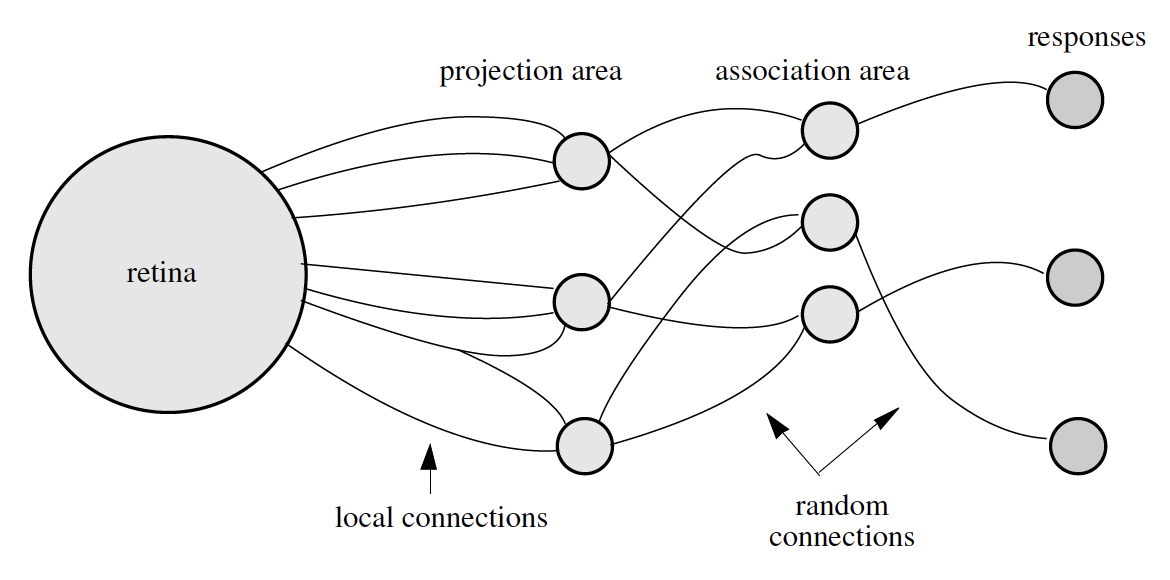
\includegraphics[scale=0.4]{Figures/nn_3.1.png}
		%	\caption{John Urbanic, Pittsburgh Supercomputing Center}
	\end{figure}	
	
	
\end{frame}

\begin{frame}{Threshold logic}
	The computational equivalent is a network with weights $w_i$ and a number of input units $P_i$. If the combined value of the inputs is larger than $\theta$, then it fires a 1, otherwise a 0.

			\begin{figure}[h]
	\centering
	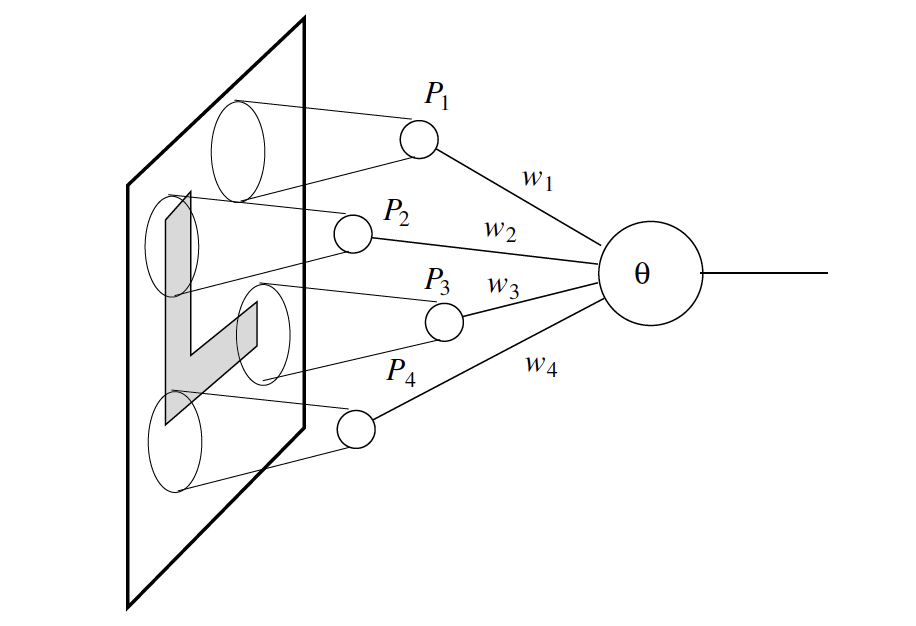
\includegraphics[scale=0.4]{Figures/nn_3.2.png}
	%	\caption{John Urbanic, Pittsburgh Supercomputing Center}
\end{figure}	
	
	
\end{frame}

\begin{frame}{Deep Neural Networks}
			\begin{figure}[h]
	\centering
	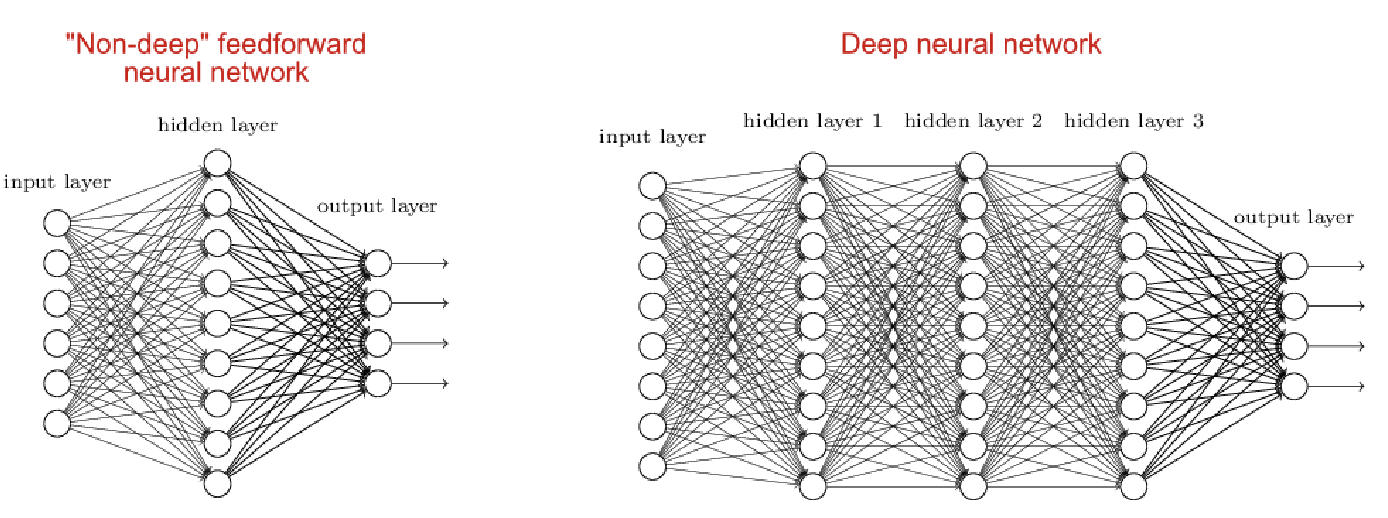
\includegraphics[scale=0.4]{Figures/fig_deep_nn.png}
	%	\caption{John Urbanic, Pittsburgh Supercomputing Center}
\end{figure}		
\end{frame}

\begin{frame}{Deep Learning}
	
	\begin{quote}
		Deep learning achieves great power and flexibility by representing the world as a nested hierarchy of concepts, with each concept defined in relation to simpler concepts and more abstract representations computed in terms of less abstract ones.
		
		Goodfellow et al. 
	\end{quote}
	


Deep  learning is only possible because of the advances in computer power (GPUs in particular). The basic concepts date back to then end of 1990's with Y. LeCun and colleagues. 
\end{frame}

\begin{frame}{Deep Learning in real time}
	One impressive representation of deep learning applied to a classification problem. This is an extension of the famous MINST digit recognition problem. 
	
	\url{https://adamharley.com/nn_vis/mlp/3d.html}
	
\end{frame}

\begin{frame}{Deep Learning Methods}
Every DL method relies on a specific design (architecture) and purpose
	\begin{figure}[h]
		\centering
		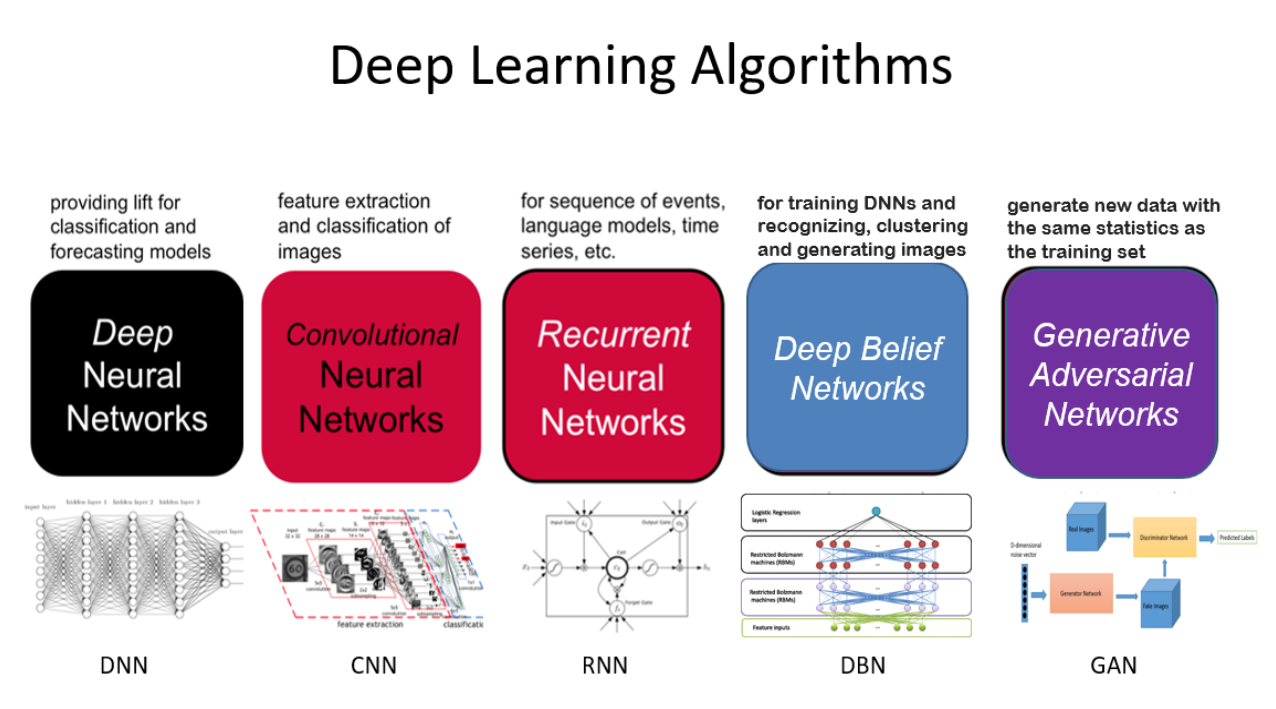
\includegraphics{Figures/DLalgorithms.png}
	\end{figure}	
\end{frame}

	\begin{frame}{Understanding, Interpreting, Explaining}
	\begin{itemize}
		\item Understanding a model $\Rightarrow$ characterizing a model’s behavior without  elucidating its internal mechanisms
		\item Interpreting a model $\Rightarrow$ rendering the algorithms decision-making process in terms a human expert can comprehend
		\item Explaining a model $\Rightarrow$ defining the collection of features (usually in the input) that are most significant in producing the algorithm’s output
		
	\end{itemize}
Holzinger et al. arXiv:1712.09923 (2017). 
	
\end{frame}

\begin{frame}{Visual Explainability in CNN}

	\begin{figure}[h]
	\centering
	\small{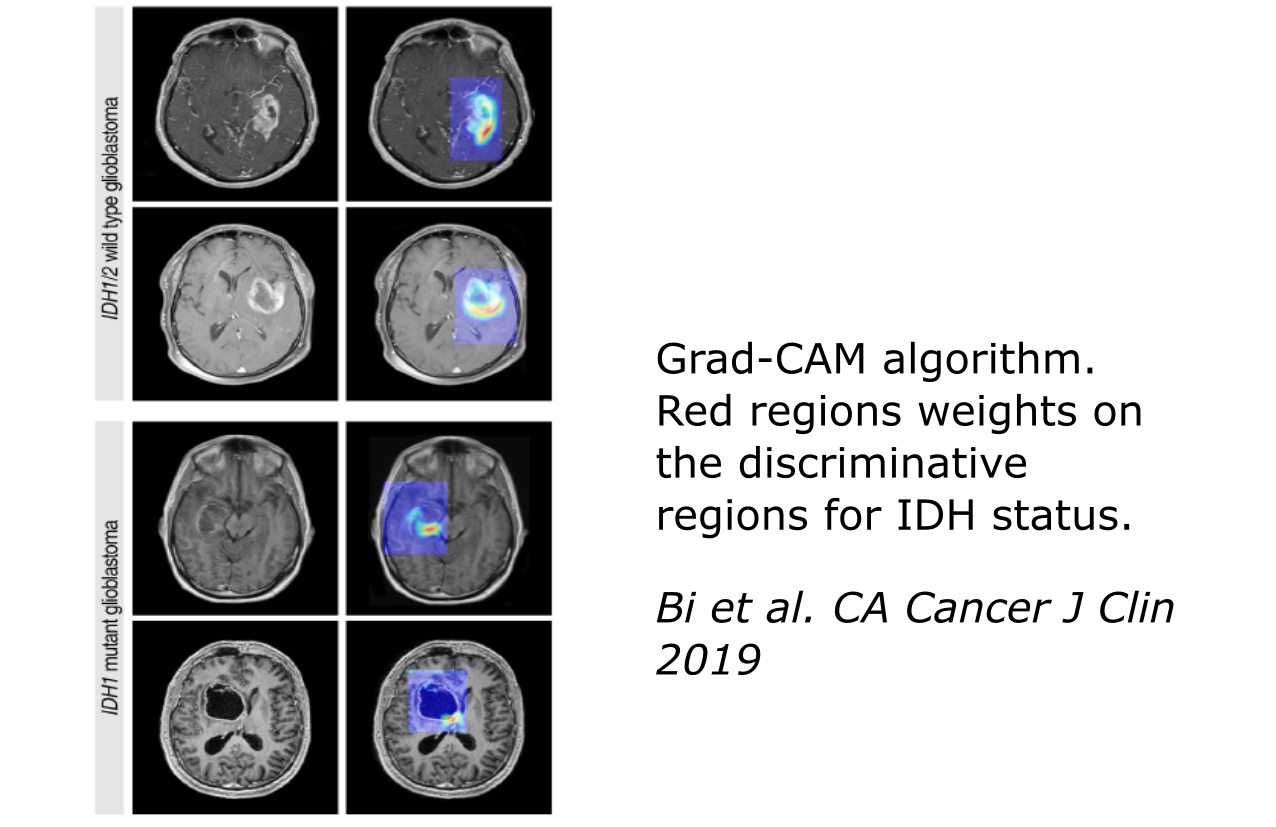
\includegraphics{Figures/explaincnn.png}}
\end{figure}	

\end{frame}
\begin{frame}{Deep Learning pitfalls}
	Applications of deep learning and architectures is abundant, and results really impressive. 
	However, there are still some fundamental theoretical problems that have not been solved.
	For instance the \textbf{Black box problem} in which is not clear how the deep neural network makes decisions and how can it be modified.  
\end{frame}



\section{TCIA}	

\begin{frame}{The Cancer Imaging Archive}
	UAMS hosts \hyperlink{https://www.cancerimagingarchive.net/}{the Cancer Imaging Archive}
	\begin{figure}[h]
		\centering
		
\includegraphics[scale=0.45]{Figures/TCIA.png}
		%\caption{Fig 15: CORD-19 challenge}
	\end{figure}
	
\end{frame}


\section{Imaging Research}
	

	
	\begin{frame}{What do I do in DBMI?}
		I have research projects in:
		\begin{itemize}
			\item Statistical Machine Learning
			\item Functional and Elastic Shape Analysis
			\item Deep Learning in imaging
			\item Neuro-imaging			
			\item Cancer genomics/imaging data integration
			\item Limb Development
		\end{itemize}
		
	\end{frame}

\begin{frame}{Imaging Research}
	
	\begin{figure}[h]
		\centering
		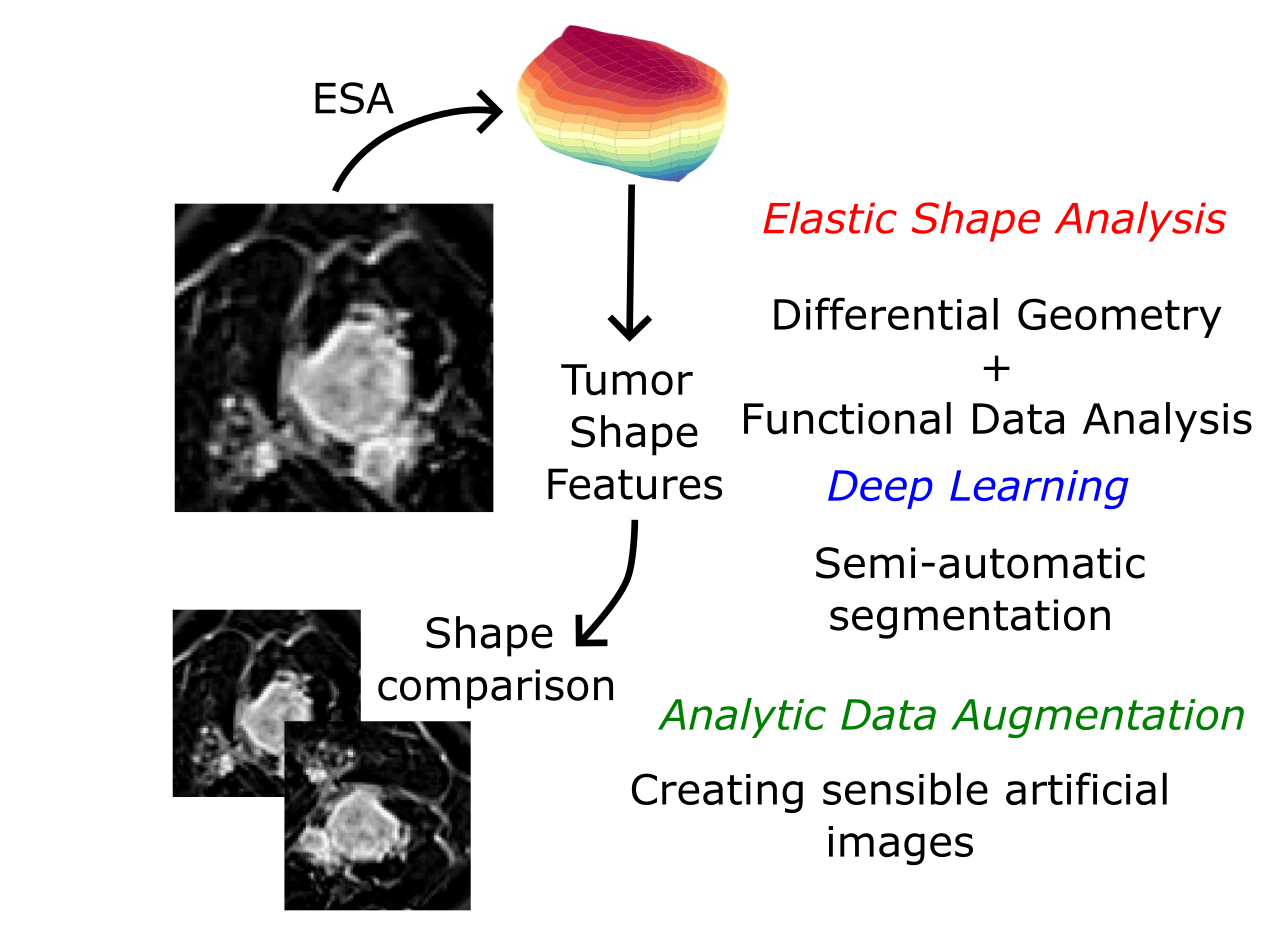
\includegraphics{Figures/hgresearch.png}
		%\caption{Computer/Scripting Languages}
	\end{figure}
	
\end{frame}
	\begin{frame}{Bioinformatics }
		
		\begin{figure}[h]
			\centering
			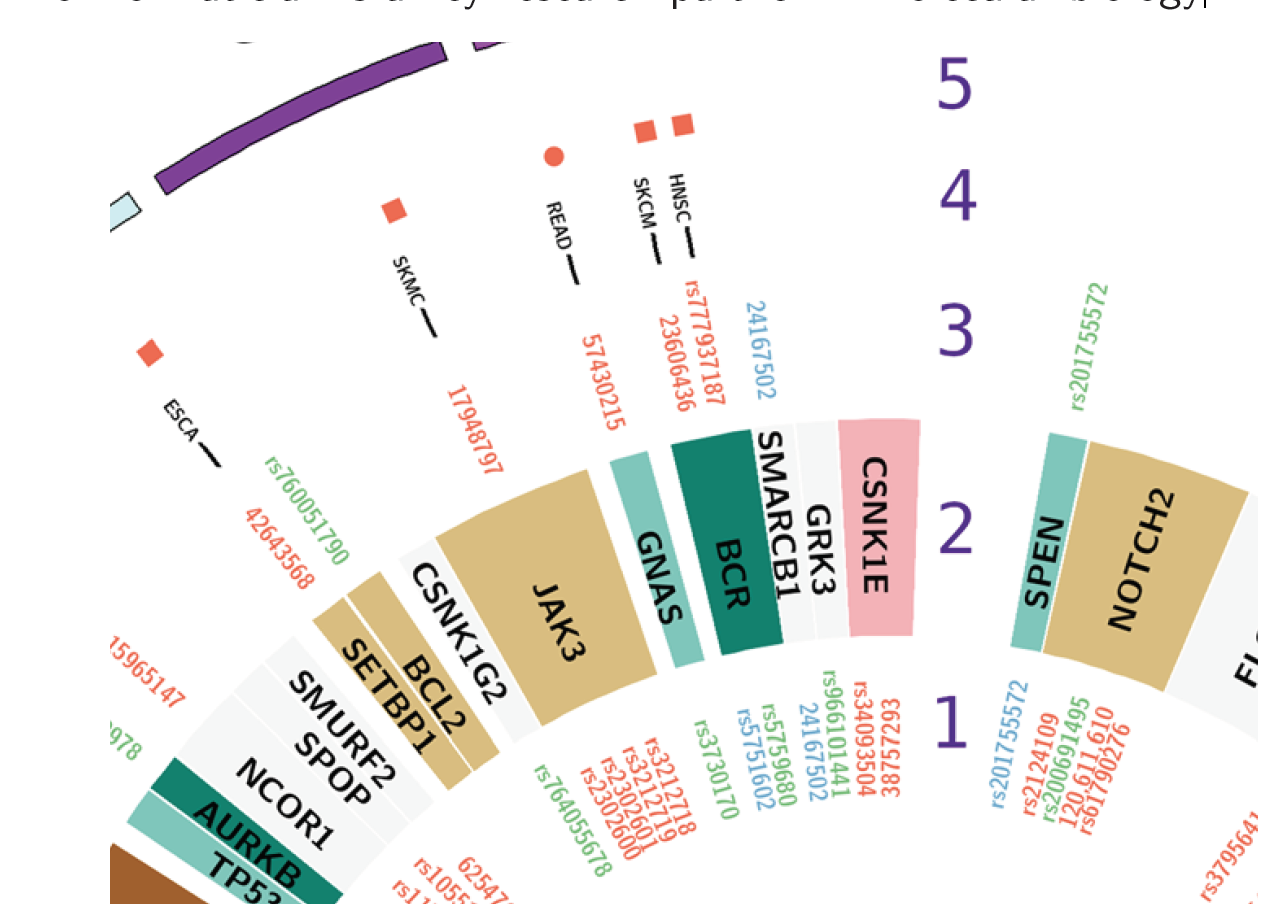
\includegraphics[scale=0.45]{Figures/analyz.png}
			%\caption{Computer/Scripting Languages}
		\end{figure}
		
		
	\end{frame}
	
\section{Final pitch for collaborating with DBMI}
\begin{frame}{DBMI is highly interdisciplinary}

	\begin{figure}[h]
		\centering
		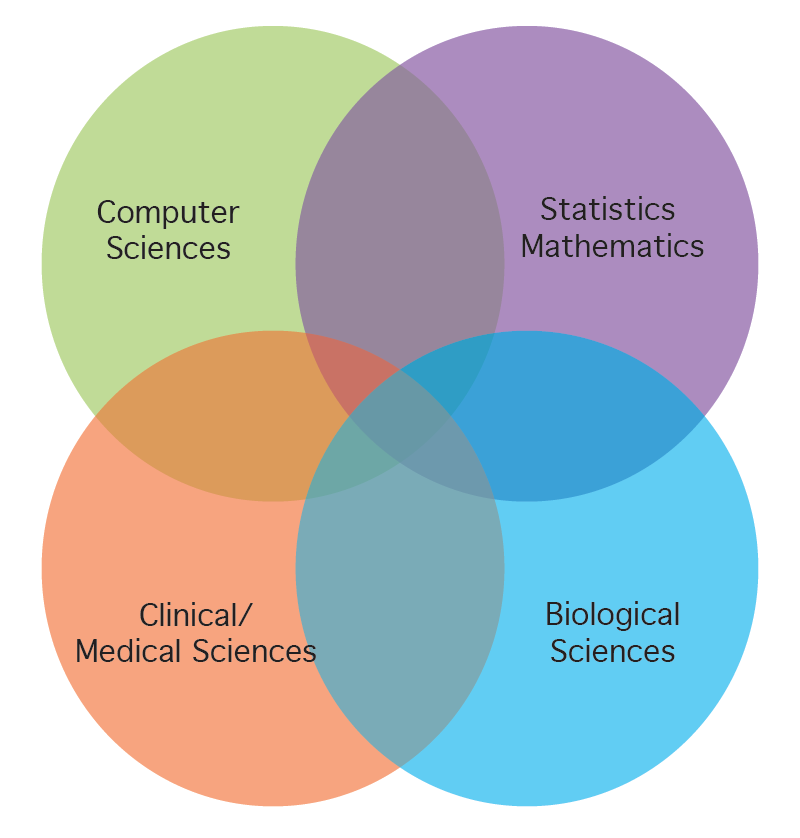
\includegraphics[scale=0.45]{Figures/venn.png}
		%\caption{Scientific Areas in BMI}
	\end{figure}
	
\end{frame}


\begin{frame}{What computer language do I need?}
	It really depends on the area that you want to specialize and your
	background. At DBMI, all our students must acquire certain competency in
	Python
	\begin{figure}[h]
		\centering
		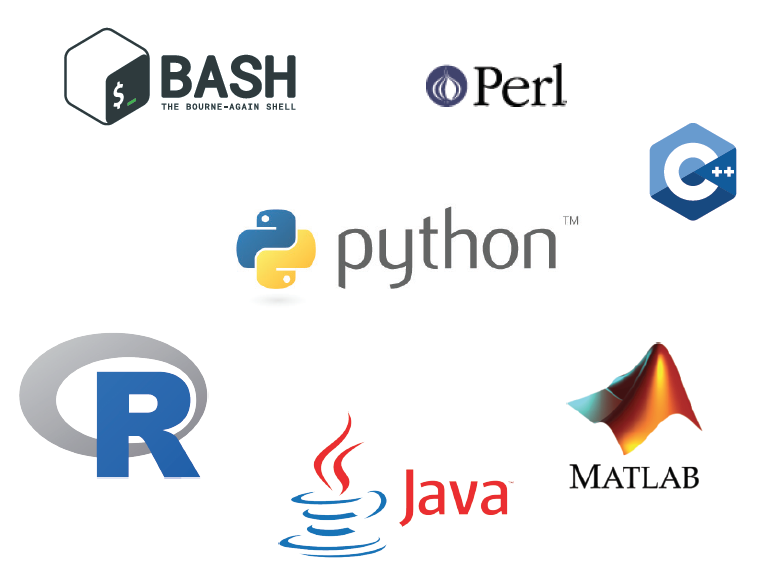
\includegraphics[scale=0.45]{Figures/languages.png}
		\caption{Computer/Scripting Languages}
	\end{figure}
	
\end{frame}

	
	\begin{frame}{Figure credits}
		Some figures come from James et al. An introduction to statistical learning, and G. Rojas, Neural Networks, both from Springer Verlag. 
		
		Dr. Fred Prior kindly shared the image on Deep Learning Algorithms from our Machine Learning lecture series.

%			\item Figure 1. \hyperlink{https://www.sciencephoto.com/media/222783/view}{Science Photo Library}
%			\item Figure 2. \hyperlink{https://www.nature.com/scitable/topicpage/discovery-of-dna-structure-and-function-watson-397/}{Nature Education}
%			\item Figure 3. 
%			\hyperlink{https://ib.bioninja.com.au/standard-level/topic-2-molecularbiology/
%				27-dna-replication-transcri/central-dogma.html}{National Human Genome Research Institute}
%			\item Figure 4. \hyperlink{https://doi.org/10.1016/j.ajhg.2018.11.014}{Integrating Genomics into Healthcare: A Global Responsibility}
%			\item Figure 6 \hyperlink{https://www.nature.com/articles/527S2a.pdf}{Big Data-The power of petabytes}
%			\item Figure 7 \hyperlink{https://dx.doi.org/10.1038/nprot.2017.149}{Exponential scaling of single-cell RNA-seq in the past decade}
%			\item Figure 8. \hyperlink{https://doi.org/10.1186/s13059-019-1724-1}{Genomics and data science: an application within an umbrella}
%			\item Figure 11 \hyperlink{http://www.biomedcentral.com/1471-2105/13/238}{Mapping single molecule sequencing reads using basic local
%				alignment with successive refinement BLASR: application and theory}
%			\item Figure 12. \hyperlink{https://doi.org/10.1038/ng.806}{ A Framework for Variation Discovery and Genotyping Using
%				Next-Generation DNA Sequencing Data}

		
	\end{frame}
	
%	\begin{frame}{Figure credits}
%		
%		\begin{itemize}
%			\item Figure 13.\hyperlink{https://cloud.google.com/life-sciences}{ Google Cloud Architecture}
%			\item Figure 14. \hyperlink{https://dcc.icgc.org/pcawg}{ ICGC Data Portal}
%			\item Figure 19. \hyperlink{https://doi.org/10.1016/j.jmir.2019.09.005}{ Machine Learning and Deep Learning in Medical Imaging:
%				Intelligent Imaging}
%			\item Figure 20. \hyperlink{https://doi.org/10.1093/jamia/ocx033}{ A longitudinal analysis of data quality in a large pediatric
%				data research network}
%			\item Figure 21. \hyperlink{https://proteomics.cancer.gov/programs/cptac}{ CPTAC}
%		\end{itemize}	
%		
%	\end{frame}
	
\end{document}